\documentclass{article}[18pt]
\ProvidesPackage{format}
%Page setup
\usepackage[utf8]{inputenc}
\usepackage[margin=0.7in]{geometry}
\usepackage{parselines} 
\usepackage[english]{babel}
\usepackage{fancyhdr}
\usepackage{titlesec}
\hyphenpenalty=10000

\pagestyle{fancy}
\fancyhf{}
\rhead{Sam Robbins}
\rfoot{Page \thepage}

%Characters
\usepackage{amsmath}
\usepackage{amssymb}
\usepackage{gensymb}
\newcommand{\R}{\mathbb{R}}

%Diagrams
\usepackage{pgfplots}
\usepackage{graphicx}
\usepackage{tabularx}
\usepackage{relsize}
\pgfplotsset{width=10cm,compat=1.9}
\usepackage{float}

%Length Setting
\titlespacing\section{0pt}{14pt plus 4pt minus 2pt}{0pt plus 2pt minus 2pt}
\newlength\tindent
\setlength{\tindent}{\parindent}
\setlength{\parindent}{0pt}
\renewcommand{\indent}{\hspace*{\tindent}}

%Programming Font
\usepackage{courier}
\usepackage{listings}
\usepackage{pxfonts}

%Lists
\usepackage{enumerate}
\usepackage{enumitem}

% Networks Macro
\usepackage{tikz}


% Commands for files converted using pandoc
\providecommand{\tightlist}{%
	\setlength{\itemsep}{0pt}\setlength{\parskip}{0pt}}
\usepackage{hyperref}

% Get nice commands for floor and ceil
\usepackage{mathtools}
\DeclarePairedDelimiter{\ceil}{\lceil}{\rceil}
\DeclarePairedDelimiter{\floor}{\lfloor}{\rfloor}

% Allow itemize to go up to 20 levels deep (just change the number if you need more you madman)
\usepackage{enumitem}
\setlistdepth{20}
\renewlist{itemize}{itemize}{20}

% initially, use dots for all levels
\setlist[itemize]{label=$\cdot$}

% customize the first 3 levels
\setlist[itemize,1]{label=\textbullet}
\setlist[itemize,2]{label=--}
\setlist[itemize,3]{label=*}

% Definition and Important Stuff
% Important stuff
\usepackage[framemethod=TikZ]{mdframed}

\newcounter{theo}[section]\setcounter{theo}{0}
\renewcommand{\thetheo}{\arabic{section}.\arabic{theo}}
\newenvironment{important}[1][]{%
	\refstepcounter{theo}%
	\ifstrempty{#1}%
	{\mdfsetup{%
			frametitle={%
				\tikz[baseline=(current bounding box.east),outer sep=0pt]
				\node[anchor=east,rectangle,fill=red!50]
				{\strut Important};}}
	}%
	{\mdfsetup{%
			frametitle={%
				\tikz[baseline=(current bounding box.east),outer sep=0pt]
				\node[anchor=east,rectangle,fill=red!50]
				{\strut Important:~#1};}}%
	}%
	\mdfsetup{innertopmargin=10pt,linecolor=red!50,%
		linewidth=2pt,topline=true,%
		frametitleaboveskip=\dimexpr-\ht\strutbox\relax
	}
	\begin{mdframed}[]\relax%
		\centering
		}{\end{mdframed}}



\newcounter{lem}[section]\setcounter{lem}{0}
\renewcommand{\thelem}{\arabic{section}.\arabic{lem}}
\newenvironment{defin}[1][]{%
	\refstepcounter{lem}%
	\ifstrempty{#1}%
	{\mdfsetup{%
			frametitle={%
				\tikz[baseline=(current bounding box.east),outer sep=0pt]
				\node[anchor=east,rectangle,fill=blue!20]
				{\strut Definition};}}
	}%
	{\mdfsetup{%
			frametitle={%
				\tikz[baseline=(current bounding box.east),outer sep=0pt]
				\node[anchor=east,rectangle,fill=blue!20]
				{\strut Definition:~#1};}}%
	}%
	\mdfsetup{innertopmargin=10pt,linecolor=blue!20,%
		linewidth=2pt,topline=true,%
		frametitleaboveskip=\dimexpr-\ht\strutbox\relax
	}
	\begin{mdframed}[]\relax%
		\centering
		}{\end{mdframed}}
\lhead{CSys}


\begin{document}
\begin{center}
\underline{\huge Sequential Circuits}
\end{center}
\section{Circuits}
\begin{center}
	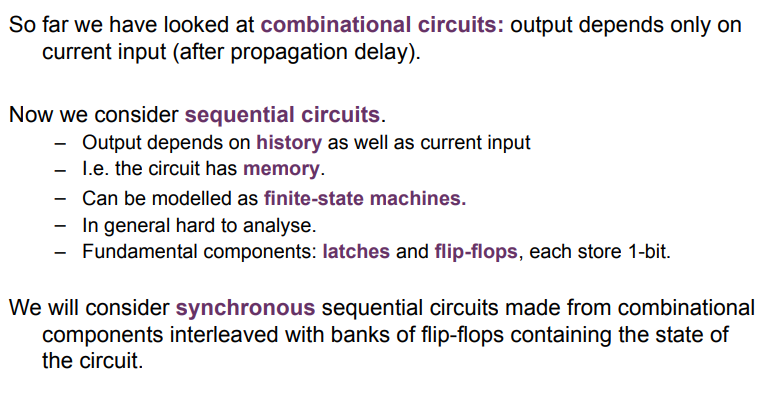
\includegraphics[scale=0.7]{figure1}
\end{center}
\section{SR Latch}
\begin{center}
	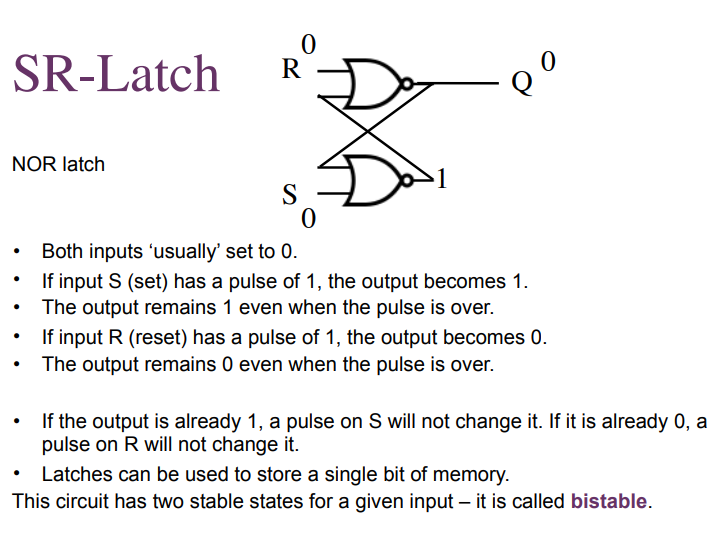
\includegraphics[scale=0.7]{figure2}
\end{center}
\begin{center}
	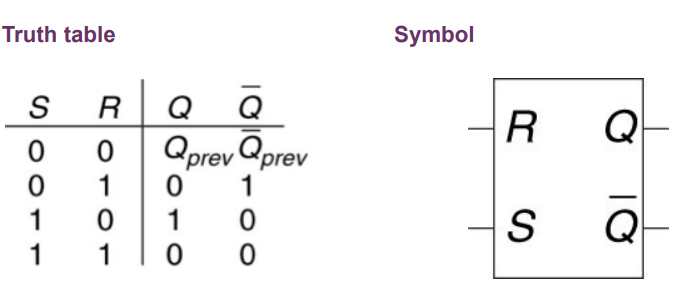
\includegraphics[scale=0.7]{figure3}
\end{center}
\begin{center}
	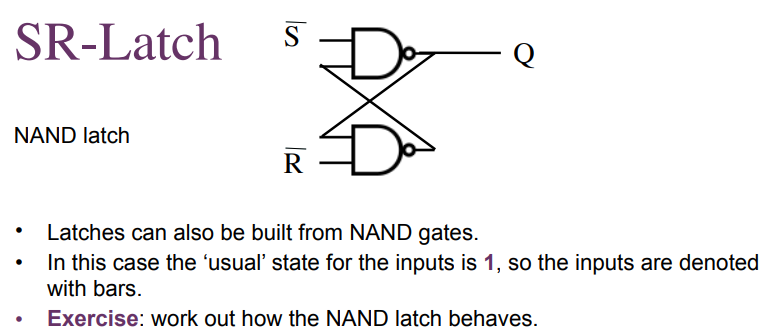
\includegraphics[scale=0.7]{figure4}
\end{center}
\section{D Latch}
\begin{center}
	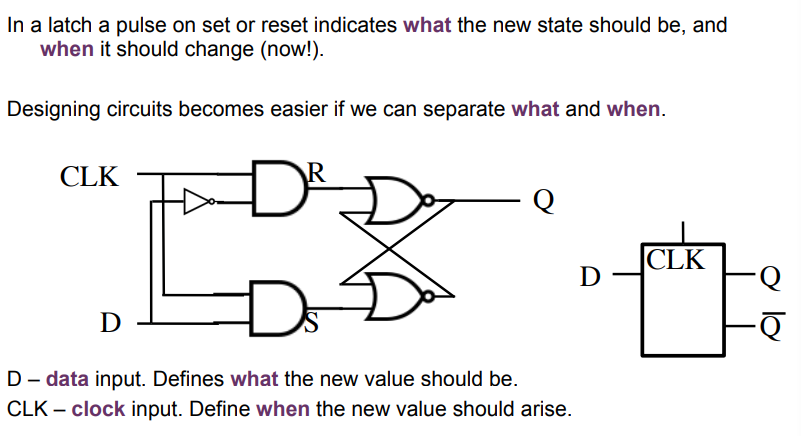
\includegraphics[scale=0.7]{figure5}
\end{center}
\begin{itemize}
	\item The output will be updated to whatever the data is whenever the clock gives a pulse
\end{itemize}
\section{D Flip Flop}
\begin{center}
	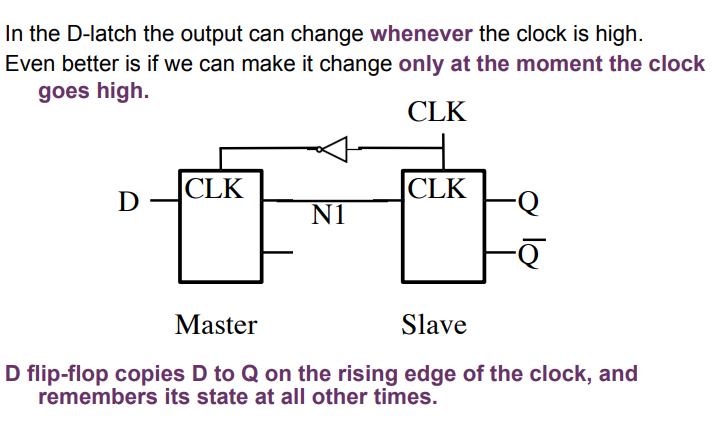
\includegraphics[scale=0.7]{figure6}
\end{center}
\begin{itemize}
	\item Whenever the clock is low, the data will transmit through the master, when the clock is high, the data will not transmit through the master
\end{itemize}
\begin{center}
	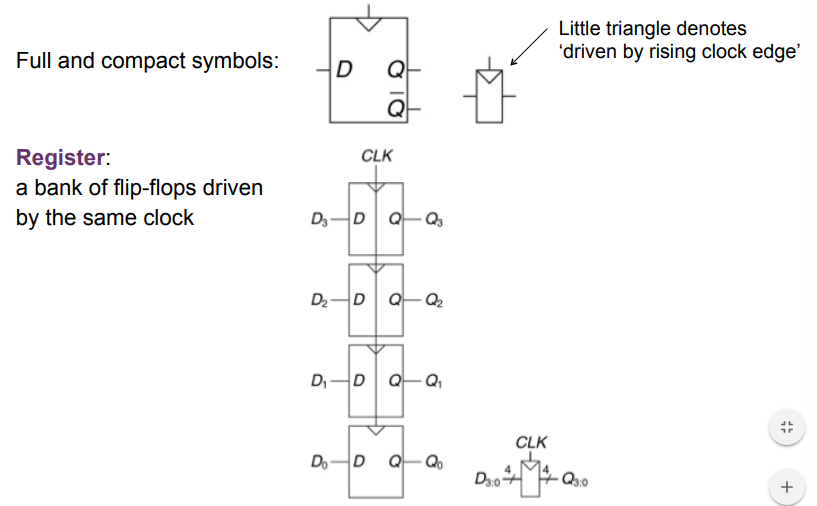
\includegraphics[scale=0.7]{figure7}
\end{center}
\section{Enabled Flip Flop}
\begin{center}
	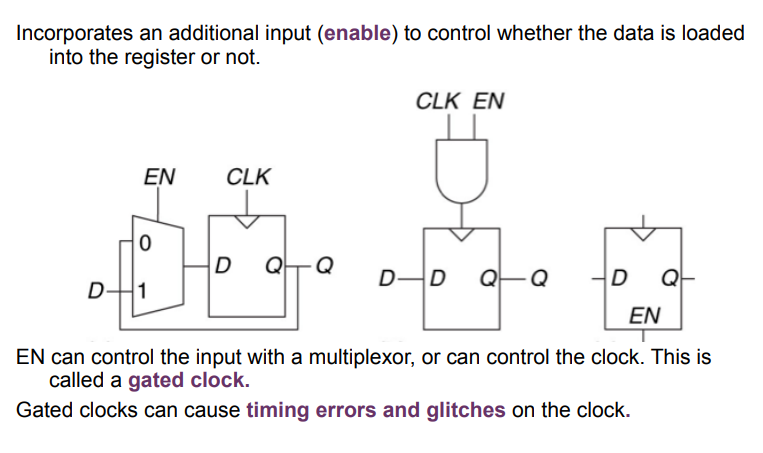
\includegraphics[scale=0.7]{figure8}
\end{center}
\begin{itemize}
	\item Therefore the 1st diagram is the best one to use as by using the end gate, timing errors can be included
\end{itemize}
\section{Flip Flop Design}
\begin{center}
	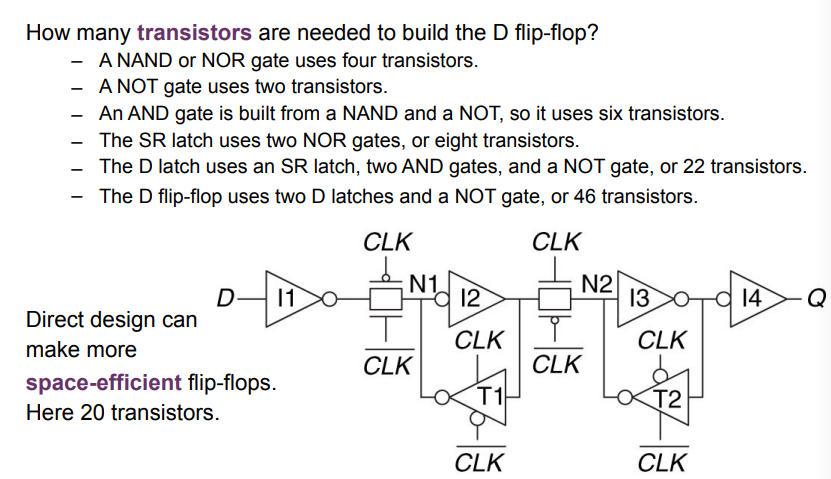
\includegraphics[scale=0.7]{figure9}
\end{center}
\section{Example}
\begin{center}
	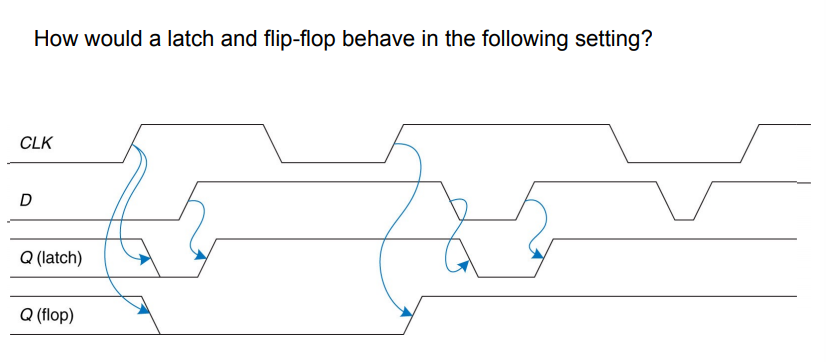
\includegraphics[scale=0.7]{figure10}
\end{center}
\section{Problem Circuits}
\begin{center}
	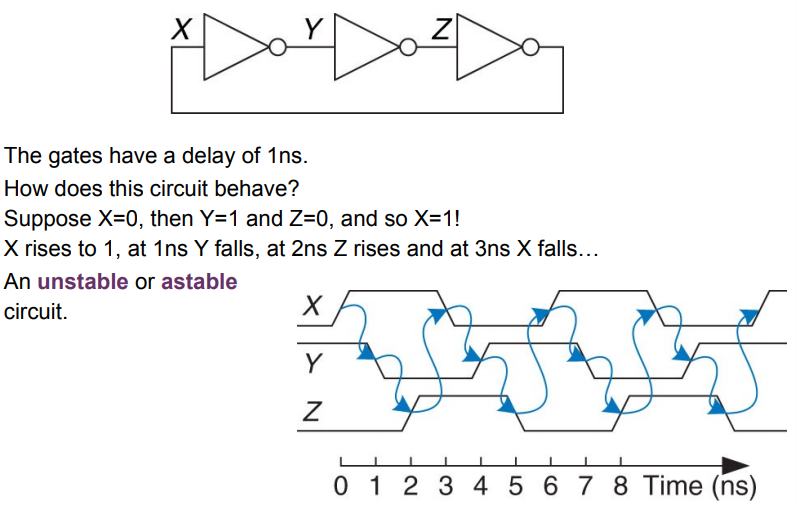
\includegraphics[scale=0.7]{figure11}
\end{center}
\begin{center}
	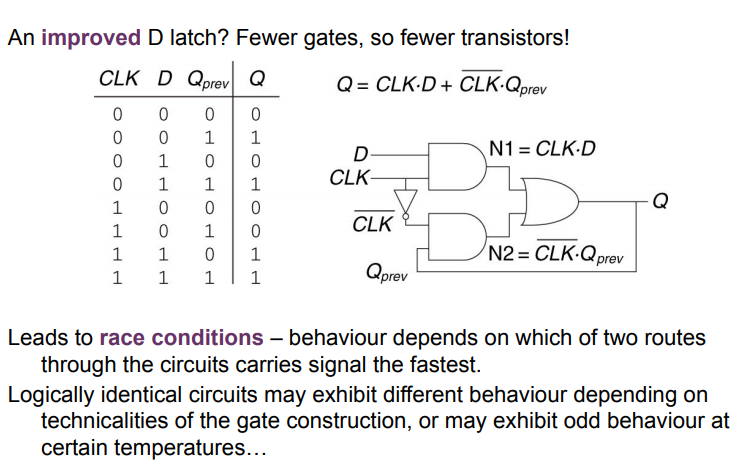
\includegraphics[scale=0.7]{figure12}
\end{center}
\begin{center}
	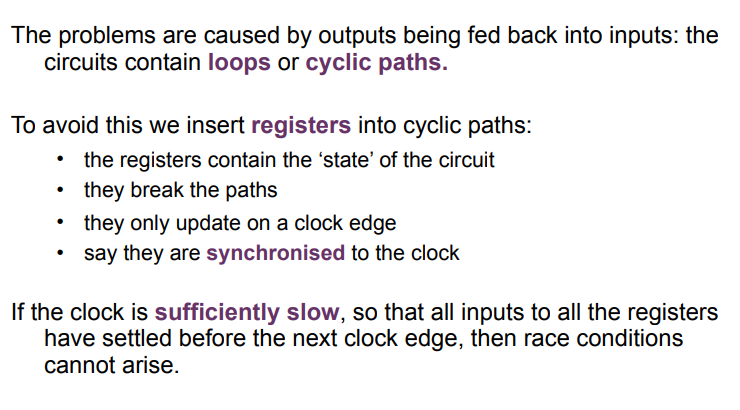
\includegraphics[scale=0.7]{figure13}
\end{center}
\section{Synchronous Circuits}
\begin{center}
	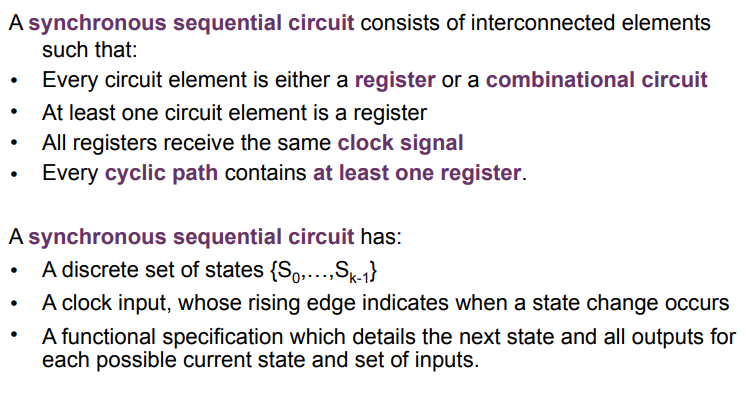
\includegraphics[scale=0.7]{figure14}
\end{center}
\section{Examples}
\begin{center}
	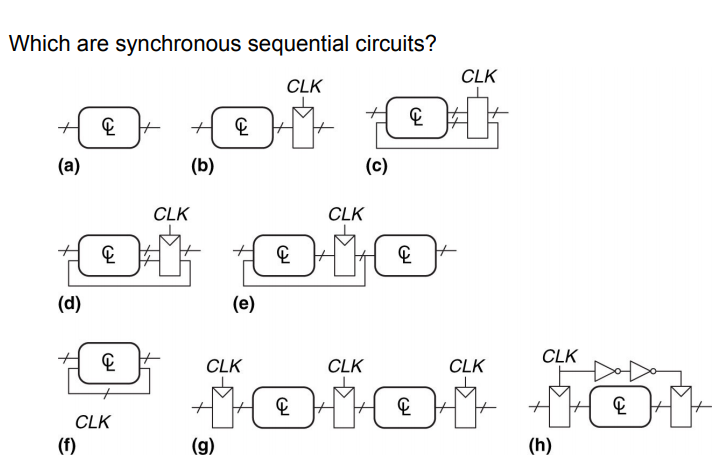
\includegraphics[scale=0.7]{figure15}
\end{center}
b,d,e,g,
\section{Timing}
\begin{center}
	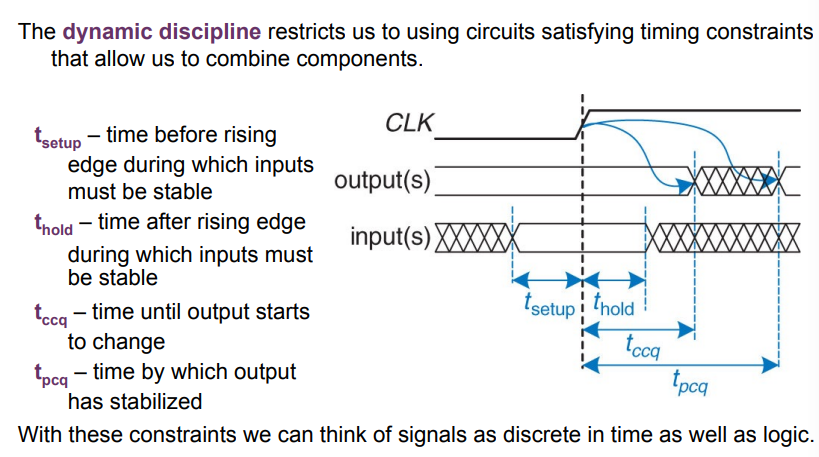
\includegraphics[scale=0.7]{figure16}
\end{center}
\begin{itemize}
	\item ccq - contamination clock to q
	\item pcq - propagation clock to q
\end{itemize}
\section{Setting Time}
\begin{center}
	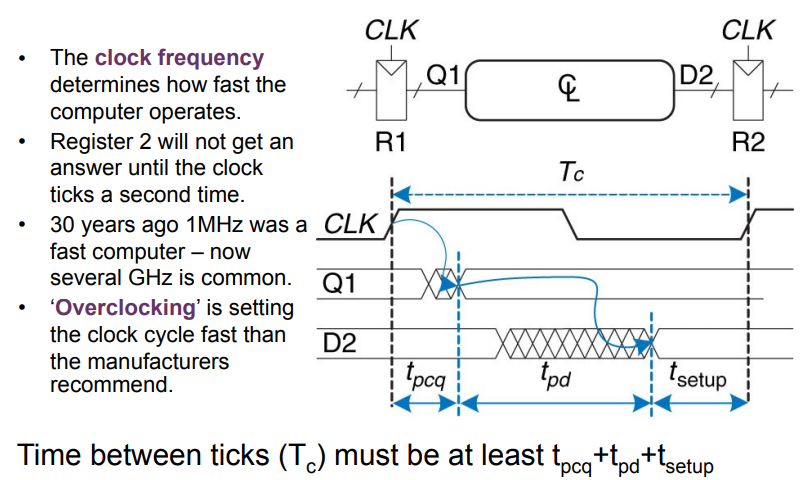
\includegraphics[scale=0.7]{figure17}
\end{center}
\begin{center}
	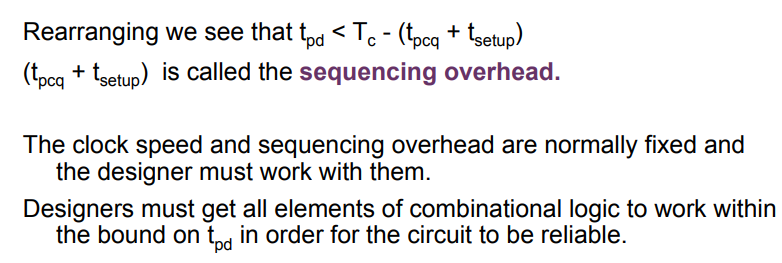
\includegraphics[scale=0.7]{figure18}
\end{center}
\begin{center}
	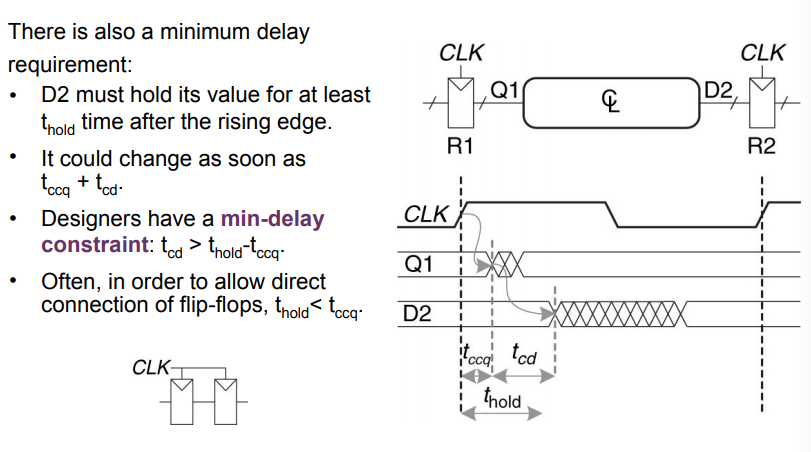
\includegraphics[scale=0.7]{figure19}
\end{center}
\section{Example}
\begin{center}
	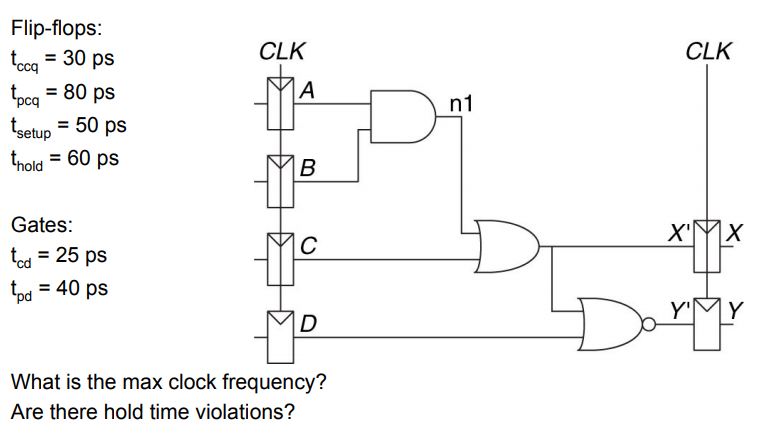
\includegraphics[scale=0.7]{figure20}
\end{center}
\begin{itemize}
	\item Critical path goes through all 3 gates
	\begin{itemize}
		\item $CL_{pd}=120ps$
	\end{itemize}
	\item $T_c\geqslant80+120+50=250ps$
	\item $1/250ps$ = 4GHz
\end{itemize}
There would be a hold time violation


\section{Fixing the hold time violation}
\begin{center}
	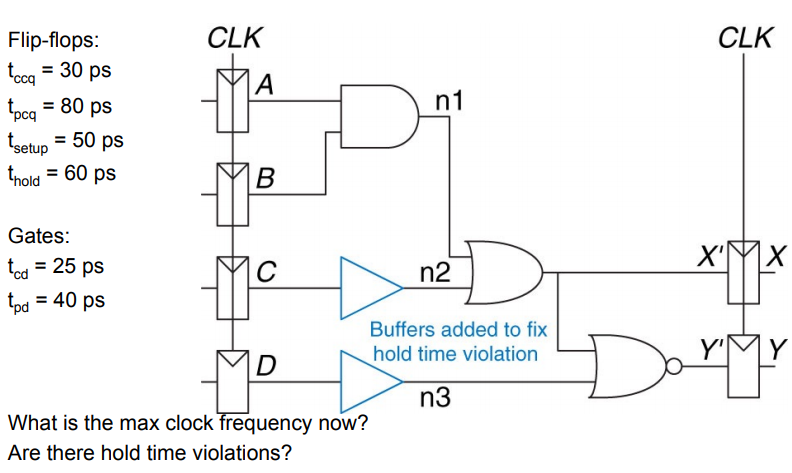
\includegraphics[scale=0.7]{figure21}
\end{center}
\section{Metastable States}
\begin{center}
	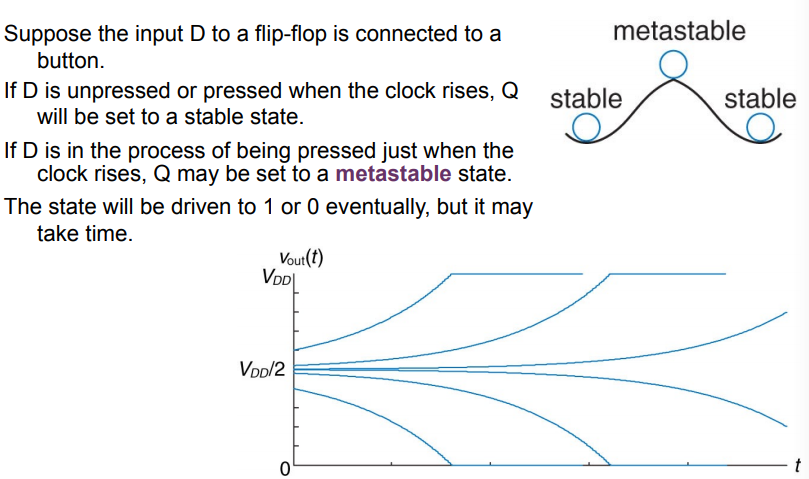
\includegraphics[scale=0.7]{figure22}
\end{center}
\section{Synchronisers}
\begin{center}
	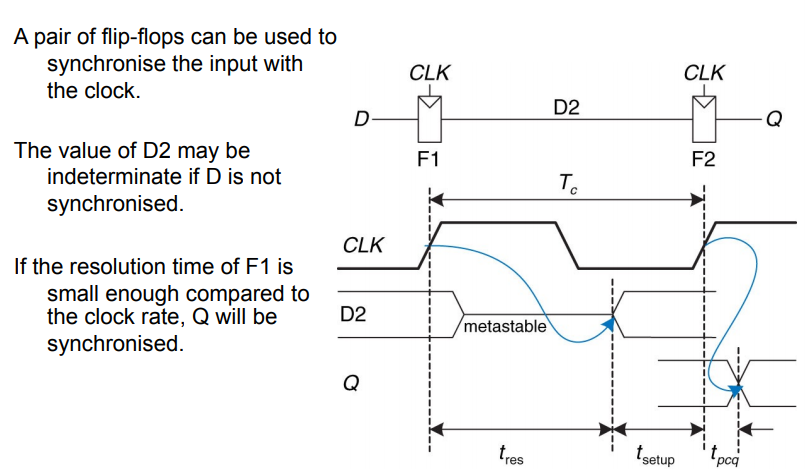
\includegraphics[scale=0.7]{figure23}
\end{center}
\section{Pipelining}
\begin{center}
	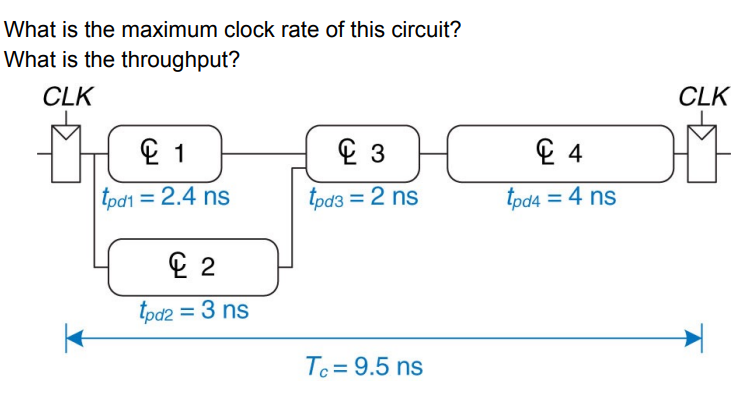
\includegraphics[scale=0.7]{figure24}
\end{center}
\begin{center}
	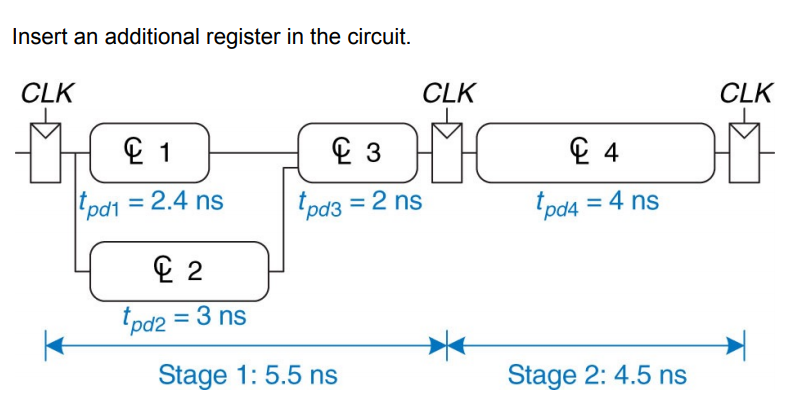
\includegraphics[scale=0.7]{figure25}
\end{center}
\begin{center}
	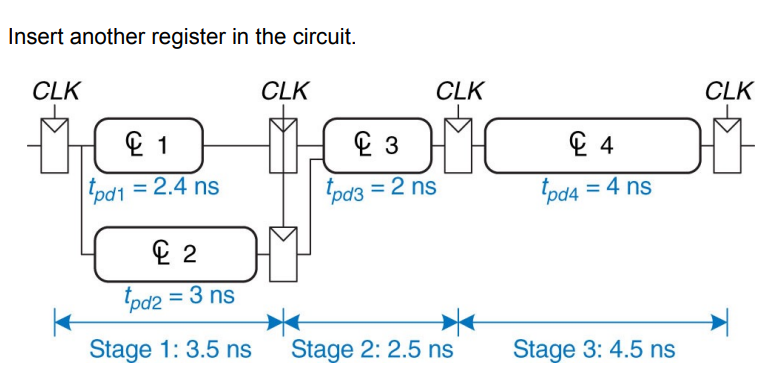
\includegraphics[scale=0.7]{figure26}
\end{center}
\begin{itemize}
	\item Doing this gives higher latency, but greater throughput
\end{itemize}



\end{document}